\documentclass[10pt,a4paper,hidelinks]{article}
\usepackage[utf8]{inputenc}
\usepackage[english]{babel}
\usepackage[T1]{fontenc}

\newcommand{\documentStatus}{DRAFT}


\usepackage{amsmath}
\usepackage{amsfonts}
\usepackage{amssymb}
\usepackage{graphicx}
\usepackage{lmodern}
\usepackage{tikz}
\usetikzlibrary{positioning}
\usetikzlibrary{shapes,snakes}
\usepackage{epigraph} 
\usepackage[left=2.5cm,
            right=2.5cm,
            top=2cm,
            bottom=2cm]{geometry}
\usepackage{setspace}
\usepackage{caption}
\usepackage{subcaption}
\usepackage{epigraph}
\usepackage{pdflscape}
\usepackage{pgfplots}

\usepackage{titlesec}
\usepackage{tcolorbox}
\usepackage{background}
\usepackage{url}
\usepackage[pdfauthor={Pierre Jézégou},
            pdftitle={ADS assignement},
            pdfsubject={Word games},
            pdfkeywords={}]{hyperref}
\usepackage{wrapfig}

\backgroundsetup{contents=\documentStatus, color=\watermarkColor}

\usepackage{fancyhdr}
\usepackage{textpos}
\usepackage{sectsty}
\usepackage{xcolor}

\setlength{\parindent}{0pt}

%%%%%%%%%%%%%%% Colors %%%%%%%%%%%%%%%
\subsectionfont{\color{fib_red}}
\subsubsectionfont{\color{fib_red}}
\renewcommand\fbox{\fcolorbox{black}{fib_red!20}}

\definecolor{fib_red}{RGB}{191,21,64}
\definecolor{fib_gray}{RGB}{111,111,111}
\definecolor{blue_upc}{RGB}{52,120,186}
\definecolor{dark_green}{rgb}{0.0, 0.4, 0.0}

\usepackage{listings}
\lstdefinestyle{mystyle}{
  backgroundcolor=\color{gray!10},
  stringstyle=\color{green!50!black},
  keywordstyle=\color{fib_red},
  numberstyle=\tiny\color{fib_gray},
  commentstyle=\color{blue_upc},
  basicstyle=\ttfamily\footnotesize,
  breakatwhitespace=false,         
  breaklines=true,                 
  captionpos=b,                    
  keepspaces=true,                 
  numbers=left,                    
  numbersep=5pt,                  
  showspaces=false,                
  showstringspaces=false,
  showtabs=false,                  
  tabsize=2
}

\lstset{style=mystyle}

\usepackage[Bjornstrup]{fncychap}
\newcommand{\watermarkColor}{red!10}


\onehalfspacing


\newcommand\VRule[1][\arrayrulewidth]{\vrule width #1}
\usepackage{xcolor,colortbl}

\newtcolorbox{mybox}[1]{
    arc=5pt,
    boxrule=0pt,
    colback=#1,
    width=\linewidth,
    halign=left,
}

\newenvironment{framed}[3]{
    \vspace*{0.5em}
    \begin{mybox}{#3!10}
        \textbf{#1}:\hfill \textit{#2}\\
        \hrule\vspace*{1em}
}
{\end{mybox}}

\newenvironment{exercise_description}[1]{
    \begin{framed}{Exercise description}{#1}{orange}
}
{\end{framed}}

\newenvironment{summary}{
    \begin{framed}{Summary}{Section \thesection}{blue}
}
{\end{framed}}


\newcommand{\colorverb}[2]{\textcolor{#1}{\texttt{\detokenize{#2}}}}
\newcommand{\type}[1]{\colorverb{green!50!black}{#1}}
\newcommand{\code}[1]{\colorverb{dark_green}{#1}}


\usepackage{lmodern}
\renewcommand*\familydefault{\sfdefault}
\usepackage{todonotes}

\fancyfoot[R]{\raisebox{-0.5\baselineskip}{
\includegraphics[scale=0.25]{images/logos/upc_logo.jpeg}}}

\begin{document}
\pagestyle{plain}
\backgroundsetup{contents=,color=red!30}
\pagecolor{white}

\begin{center}
    \color{red!50!white}
    \textbf{\huge{STATUS - \documentStatus}}
\end{center}

\vfill


\color{black}
\begin{center}
    
\includegraphics[height=2cm]{images/logos/upc_logo.jpeg} \\
    \vfill
    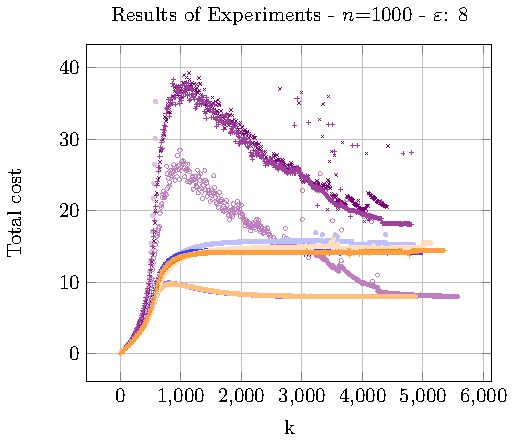
\includegraphics[width=0.6\linewidth]{includes/image_cover_page.pdf}\\
    \vfill
    \rule{\linewidth}{0.5mm} \\[1cm]
    {\Huge \textsc{\textcolor{fib_red}{Empirical Study of Union-Find}}}\\[1cm]
    {\Large \textsc{Assignment}}\\[0.4cm]
    {\huge \textsc{\textbf{Advanced data structures}}}\\[1cm]
    {\Large \textsc{Master in Research and Innovation - UPC}}\\[0.4cm]
    \rule{\linewidth}{0.5mm} \\[1.5cm]
\end{center}

\vfill

\textbf{Author:}
\begin{itemize}
\item Pierre \textsc{Jézégou}\newline
\textit{(Engineering student at École Centrale de Lille, Exchange student at UPC)}
\end{itemize}

\newpage
\color{black}
\pagecolor{white}
\pagestyle{fancy}
\tableofcontents

\section{Introduction}
\subsection{Union find}
The objective of this assignment is to implement multiple variants of the Union-Find data structure and conduct an experimental analysis of their average performance. Specifically, you will evaluate the performance of 12 different combinations by choosing one of three union strategies and one of four path compression strategies. The union strategies include unweighted quick-union (QU), union-by-size (UW), and union-by-rank (UR). The path compression strategies consist of no compression (NC), full path compression (FC), path splitting (PS), and path halving (PH). The performance assessment will involve initializing a Union-Find data structure with $n$ blocks and processing $m$ distinct pairs of elements in a random order until a single block remains. During this process, you will measure the total path length (TPL) and total pointer updates (TPU) at regular intervals.\\

\subsection{Strategy of resolution}
For each pair processed, you will calculate TPL by summing the distances of all elements to their representatives and TPU by counting the number of pointer updates required during a Find operation, depending on the path compression strategy used. The experiment will be repeated multiple times for different values of $n$ (e.g., 1000, 5000, 10000), and the results will be averaged to determine the performance of each combination. The final report should include a description of the program, the experimental setup, and plots summarizing the results. These plots should illustrate the evolution of TPL and TPU as a function of the number of pairs processed and compare different heuristics for fixed values of $n$. An optional component of the study involves measuring the actual execution times of the algorithms. The report, prepared using \LaTeX, should be submitted along with the source code and auxiliary files in a zip or tar archive by the specified deadline.

\section{Implementation}
\subsection{Data structure}
\subsubsection{Union-Find Implementation}
The Union-Find data structure is implemented to manage a dynamic set of elements partitioned into disjoint subsets. The class \code{UnionFind} is initialized with a specified number of elements $n$ and a path compression strategy. The primary attributes include \code{parents}, a list where each element points to its parent (initially itself), and \code{n_blocks}, tracking the number of disjoint sets. The class supports several path compression techniques through the \code{PathCompressionType} enumeration, including no compression (NC), full path compression (FC), path splitting (PS), and path halving (PH).

The \code{find} method identifies the representative of the set containing a given element, applying the specified path compression strategy to optimize future operations. The \code{merge} method unites two sets by linking their representatives, thus reducing the number of disjoint sets. Additional methods such as \code{tpl} and \code{tpu} compute the Total Path Length and Total Pointer Updates, respectively, providing metrics for evaluating the efficiency of the data structure. These methods iterate through all elements, calculating depths and pointer updates based on the chosen path compression technique.

\subsubsection{Class Inheritance}
To extend the functionality of the base \code{UnionFind} class, we implement specific union strategies using class inheritance. The \code{QuickUnion} class inherits from \code{UnionFind} and overrides the \code{merge} method to perform a quick union operation. In this strategy, one tree's root is attached to the other tree's root, maintaining the simplicity of the union operation.

The \code{UnionWeight} class, also inheriting from \code{UnionFind}, implements the union-by-size strategy. It modifies the \code{merge} method to attach the smaller tree to the root of the larger tree, optimizing the tree height. This is achieved by keeping track of the sizes (or weights) of the trees using negative values in the \code{parents} list.

Similarly, the \code{UnionRank} class implements the union-by-rank strategy. It overrides the \code{merge} method to attach the tree with lower rank to the tree with higher rank. This approach ensures that the resulting tree remains balanced, thereby reducing the maximum tree height. Both \code{UnionWeight} and \code{UnionRank} classes utilize the path compression strategies defined in the base class to enhance the efficiency of the \code{find} operations.

\subsection{Metrics}
\subsubsection{Total path length}
Total Path Length (TPL) is a critical metric in evaluating the efficiency of Union-Find data structures. TPL measures the cumulative distance from each element in the Union-Find structure to its representative or root. Specifically, for each element $i$, the distance $d(i)$ to its root is determined, and these distances are summed across all elements. Mathematically, TPL is defined as:

$$\text{TPL} = \sum_{i=1}^{n} d(i)$$

This metric provides insight into the overall depth and compactness of the data structure, reflecting the efficiency of union and find operations. A lower TPL indicates that elements are, on average, closer to their roots, which implies faster find operations. During the experiments, TPL is calculated at regular intervals as pairs of elements are processed and unions are performed. By analyzing TPL across different union and path compression strategies, we can determine which combinations yield more efficient Union-Find structures in terms of minimizing the overall path length.

\begin{lstlisting}[language=Python, caption=Python implementation of TPL]
def tpl(self) -> int:
    """Calculate the Total Path Length (TPL)."""
    total_path_length = 0
    for i in range(len(self.parents)):
        total_path_length += self.depth(i)
    return total_path_length
\end{lstlisting}

\subsubsection{Total pointer updates}
Total Pointer Updates (TPU) is an essential metric for assessing the efficiency of path compression strategies in Union-Find data structures. TPU measures the total number of pointer updates that occur during find operations across all elements. For each element $i$, the number of pointers updated during a find operation, $u(i)$, is counted. The TPU is then the sum of these updates for all elements. Formally, TPU is defined as:

$$\text{TPU} = \sum_{i=1}^{n} u(i)$$

For the no compression (NC) strategy, this value is always zero, as no pointers are updated. For other strategies, TPU can be computed more efficiently by knowing the number of children of each root. For instance, with full path compression (FC), TPU can be calculated as:

$$\text{TPU}_{\text{FC}} = \text{TPL} - \sum_{r \in \text{roots}} \text{number of children of } r$$

This metric reflects the effort involved in maintaining the structure's efficiency via path compression. During the experiments, TPU is calculated at regular intervals as pairs of elements are processed and unions are performed. By analyzing TPU across different union and path compression strategies, we can determine which combinations minimize the overhead associated with pointer updates, thereby enhancing the overall performance of the Union-Find structure.


\begin{description}
    \item[No Compression (NC):]
      \[
      \text{TPU}_{\text{NC}}(i) = 0
      \]
      Since no compression is applied, no pointer updates are necessary.
    
    \item[Full Path Compression (FC):]
      \[
      \text{TPU}_{\text{FC}}(i) = d(i) - 1
      \]
      Full path compression updates each node on the path to point directly to the root. Thus, each find operation updates $d(i) - 1$ pointers, where $d(i)$ is the depth of node $i$.
    
    \item[Path Splitting (PS):]
      \[
      \text{TPU}_{\text{PS}}(i) = d(i) - 1
      \]
      Path splitting updates each node on the path to point to its grandparent, resulting in $d(i) - 1$ pointer updates per find operation.
    
    \item[Path Halving (PH):]
      \[
      \text{TPU}_{\text{PH}}(i) = \left\lfloor \frac{d(i)}{2} \right\rfloor
      \]
      Path halving updates every other node on the path to point to its grandparent. Thus, the number of pointer updates per find operation is approximately half the depth, represented by $\left\lfloor \frac{d(i)}{2} \right\rfloor$.
\end{description}

Considering the recurrence formulas for each compression type, the final formula for total TPU calculation is:

\[
\text{TPU} = \sum_{i=1}^{n} 
\begin{cases} 
0 & \text{if the path compression type} = \text{NC} \\
d(i) - 1 & \text{if the path compression type} \in \{\text{FC}, \text{PS}\} \\
\left\lfloor \frac{d(i)}{2} \right\rfloor & \text{if the path compression type} = \text{PH} \\
\end{cases}
\]

This comprehensive formula captures the calculation of TPU for each path compression type used in the Union-Find data structure.

\begin{lstlisting}[language=Python, caption=Python implementation of TPU for each compression type]
def tpu(self) -> int:
    """Calculate the Total Path Updates (TPU)."""
    total_path_updates = 0
    for i in range(len(self.parents)):
        path_length = self.depth(i)
        path_updates = 0
        # no compression
        if self.path_compression_type == PathCompressionType.NC:
            path_updates = 0
        # full path compression or path splitting
        elif self.path_compression_type in (PathCompressionType.FC, PathCompressionType.PS):
            path_updates = path_length - 1 if path_length > 0 else 0
        # path halving
        elif self.path_compression_type == PathCompressionType.PH:
            path_updates = floor(path_length / 2)
        else:
            sys.stderr.write("Invalid path compression type\n")
        total_path_updates += path_updates
    return total_path_updates
\end{lstlisting}

\subsection{Total cost}
In this assignment, the total cost of the union-find data structure is calculated by processing pairs of elements and conducting unions until a single block remains. The experiment measures Total Path Length (TPL) and Total Pointer Updates (TPU) at regular intervals. The total cost is then computed using the formula:

$$\text{Total Cost} = 2 \times \text{TPL} + \varepsilon \times \text{TPU}$$

where $\varepsilon$ is a weight factor for pointer updates. This total cost metric provides a comprehensive assessment of the efficiency of different union-find strategies under various configurations.

The importance of $\varepsilon$ lies in its role in balancing the contributions of TPL and TPU to the total cost. By adjusting $\varepsilon$, we can emphasize or de-emphasize the cost of pointer updates relative to the cost of path traversal. A higher $\varepsilon$ value means that pointer updates are considered more expensive, thus strategies that minimize TPU will be favored. Conversely, a lower $\varepsilon$ value places more emphasis on minimizing TPL. This flexibility allows the total cost metric to be tailored to different scenarios and performance considerations, making it a versatile tool for evaluating union-find strategies.


\section{Experimental setup}
The objective of this experimental study is to evaluate the performance of various Union-Find data structures under different union strategies and path compression heuristics. The performance is assessed by measuring the Total Path Length (TPL) and Total Pointer Updates (TPU) during the union operations.
\subsection{Union-Find Variants}
\subsubsection{Strategies}
We consider 12 combinations of Union-Find strategies based on three union strategies and four path compression techniques:
\begin{lstlisting}[language=Python]
strategies = {
    "QU-NC": (QuickUnion, PathCompressionType.NC),
    "QU-FC": (QuickUnion, PathCompressionType.FC),
    "QU-PS": (QuickUnion, PathCompressionType.PS),
    "QU-PH": (QuickUnion, PathCompressionType.PH),
    "UW-NC": (UnionWeight, PathCompressionType.NC),
    "UW-FC": (UnionWeight, PathCompressionType.FC),
    "UW-PS": (UnionWeight, PathCompressionType.PS),
    "UW-PH": (UnionWeight, PathCompressionType.PH),
    "UR-NC": (UnionRank, PathCompressionType.NC),
    "UR-FC": (UnionRank, PathCompressionType.FC),
    "UR-PS": (UnionRank, PathCompressionType.PS),
    "UR-PH": (UnionRank, PathCompressionType.PH),
}
\end{lstlisting}

\subsubsection{Experiment Repetition and Data Collection}
The experiments are repeated $T = 20$ times for each combination of union and path compression strategies. For each repetition, we measure TPL and TPU at intervals of $\Delta$ pairs processed. The averages of TPL and TPU are then calculated for different values of $N$ (number of pairs processed).\\

\textit{Note: For convenience, we use $\Delta$ depending on the value of $N$ to reduce the number of data points and, as a consequence, reduce the time required to run the experiments.}

\subsubsection{Values of $n$ and Plotting}
The experiments are conducted for different values of $n$, specifically $n = 1000$, $n = 5000$, and $n = 10000$. For each $n$, we plot the evolution of TPL and TPU as functions of $N$, normalized by dividing TPL and TPU by $n$. This normalization gives the average distance to the root of a random node and the average number of pointers updated during a find operation.
\begin{lstlisting}[language=Python]
n_values = [1000, 5000, 10000]
T = 20
\end{lstlisting}

\subsection{Experimental Procedure}
\subsubsection{Initialization and Pair Processing}
For each combination, the Union-Find data structure is initialized with $n$ elements, each in its own block. We then process $\binom{n}{2}$ distinct pairs $(i, j)$ in random order, performing a union operation for each pair. The processing stops when there is only one block left in the structure, which typically occurs after approximately $\Theta(n \log n)$ pairs have been processed.

\subsubsection{Performance Metrics}
During the processing of pairs, we measure the following parameters:
\begin{itemize}
    \item \textbf{Total Path Length (TPL)}: The sum of distances from each element to its root.
    \item \textbf{Total Pointer Updates (TPU)}: The total number of pointers updated during the path compression.
\end{itemize}

The cost of each heuristic is evaluated using a linear combination of TPL and TPU. For example, the total cost of Full Path Compression (FC) can be expressed as $2 \cdot \text{TPL} + \varepsilon \cdot \text{TPU}$, where $\varepsilon \geq 1$ represents the cost of updating a pointer.

\subsubsection{Comparative Analysis}
To facilitate a fair comparison between different heuristics, we fix $\varepsilon = 2$ and report the total and average costs. This comparison helps in understanding the trade-offs between different union strategies and path compression techniques.

\subsubsection{Implementation and Execution}
The experiments are implemented in Python, with the full source code provided in the appendix. The code is designed to efficiently compute TPL and TPU for each configuration of the Union-Find. Detailed instructions on reproducing the experiments are provided in the README file included with the submission.

The full listing of the code and detailed explanations of the implementation are included in the appendix of this report.

\section{Results}
\subsection{Total Path Length}
\begin{description}
    \item[$N = 1000$] This plot illustrates the evolution of TPL as a function of the number of pairs processed for different union and path compression strategies. The results are averaged over $T=20$ repetitions for each combination. The TPL values are normalized by dividing by $n$ to provide a fair comparison across different values of $n$.
    \begin{figure}[h]
        \centering
        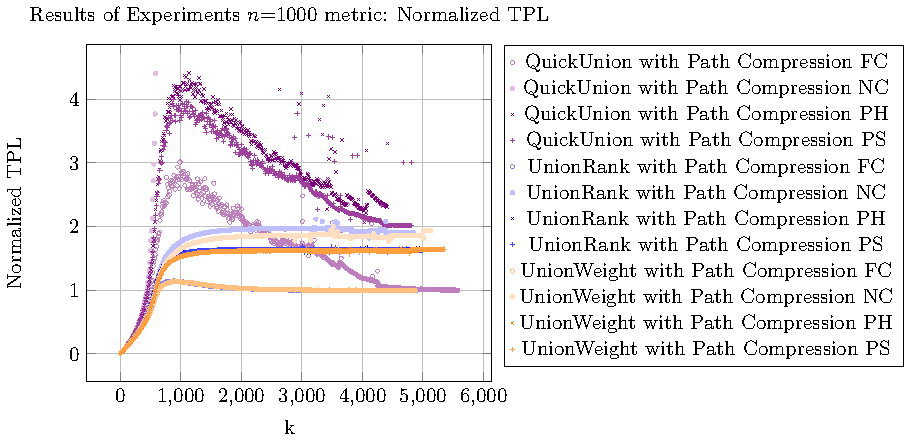
\includegraphics[width=\linewidth]{plots/plot_1000_Normalized TPL.pdf}
        \caption{Total Path Length for $n = 1000$}
    \end{figure}
    \item[$N = 5000$] Same as above, but for $n = 5000$.
    \begin{figure}[h]
        \centering
        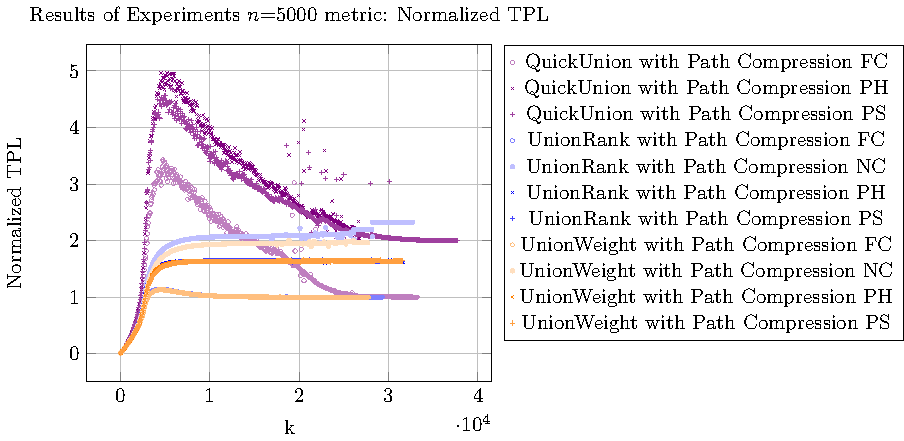
\includegraphics[width=\linewidth]{plots/plot_5000_Normalized TPL.pdf}
        \caption{Total Path Length for $n = 5000$}
    \end{figure}
    \item[$N = 10000$] Same as above, but for $n = 10000$.
    \begin{figure}[h]
        \centering
        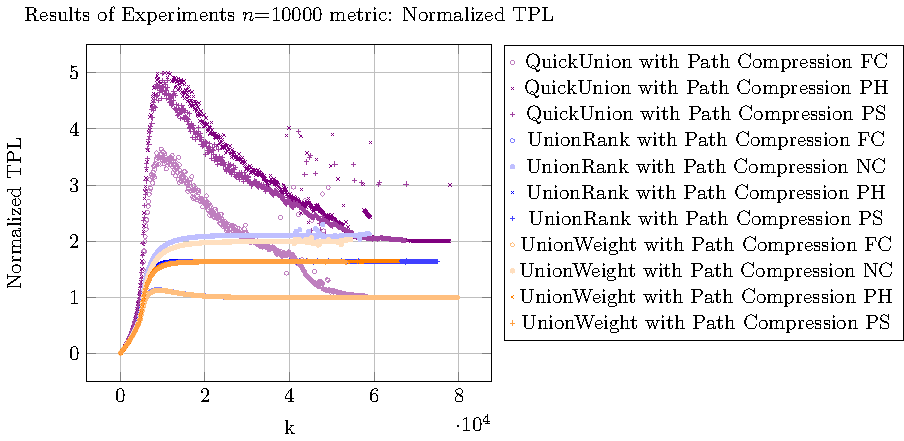
\includegraphics[width=\linewidth]{plots/plot_10000_Normalized TPL.pdf}
        \caption{Total Path Length for $n = 10000$}
    \end{figure}
\end{description}

\subsection{Total Pointer Updates}
\begin{description}
    \item[$N = 1000$] This plot illustrates the evolution of TPU as a function of the number of pairs processed for different union and path compression strategies. The results are averaged over $T=20$ repetitions for each combination. The TPL values are normalized by dividing by $n$ to provide a fair comparison across different values of $n$.
    \begin{figure}[h]
        \centering
        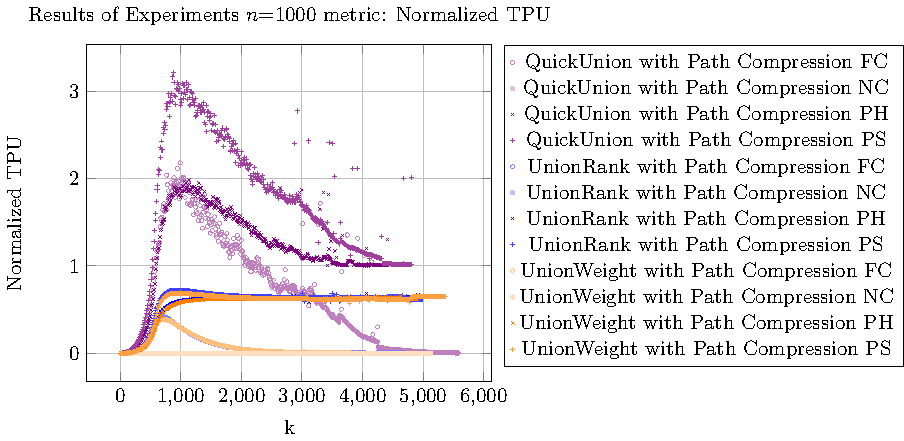
\includegraphics[width=\linewidth]{plots/plot_1000_Normalized TPU.pdf}
        \caption{Total Pointer Updates for $n = 1000$}
    \end{figure}
    \item[$N = 5000$] Same as above, but for $n = 5000$.
    \begin{figure}[h]
        \centering
        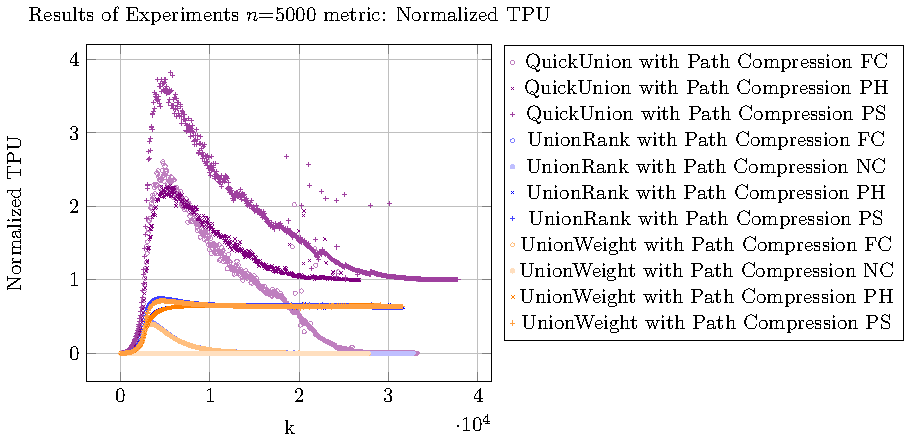
\includegraphics[width=\linewidth]{plots/plot_5000_Normalized TPU.pdf}
        \caption{Total Pointer Updates for $n = 5000$}
    \end{figure}
    \item[$N = 10000$] Same as above, but for $n = 10000$.
    \begin{figure}[h]
        \centering
        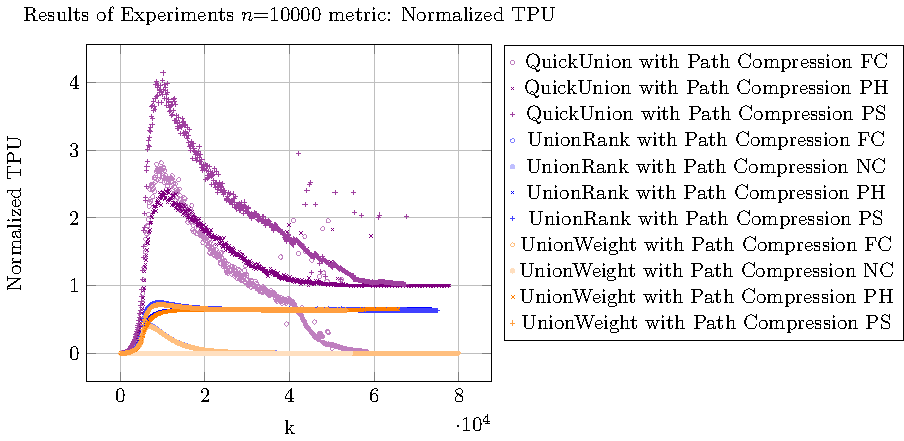
\includegraphics[width=\linewidth]{plots/plot_10000_Normalized TPU.pdf}
        \caption{Total Pointer Updates for $n = 10000$}
    \end{figure}
\end{description}

\subsection{Total cost for different heuristics}
As total cost is a linear combination of TPL and TPU, we can compare the performance of different heuristics by fixing $\varepsilon \in \{2, 5, 10, 20\}$ and calculating the total cost. The following plots illustrate the total cost for different union and path compression strategies. We just present the results for $n = 1000$ for brevity, but similar plots can be generated for $n = 5000$ and $n = 10000$. The total cost values are normalized by dividing by $n$ to provide a fair comparison across different values of $n$.
$$\boxed{\text{Total Cost}_{\text{normalized}} = \dfrac{1}{n}\left(2\times\text{TPL} + \varepsilon \times \text{TPU}\right)}$$
\begin{description}
    \item[$\varepsilon = 2$] This plot shows the total cost for different union and path compression strategies with $\varepsilon = 2$. The results are averaged over $T=20$ repetitions for each combination.
        \begin{figure}[h!]
            \centering
            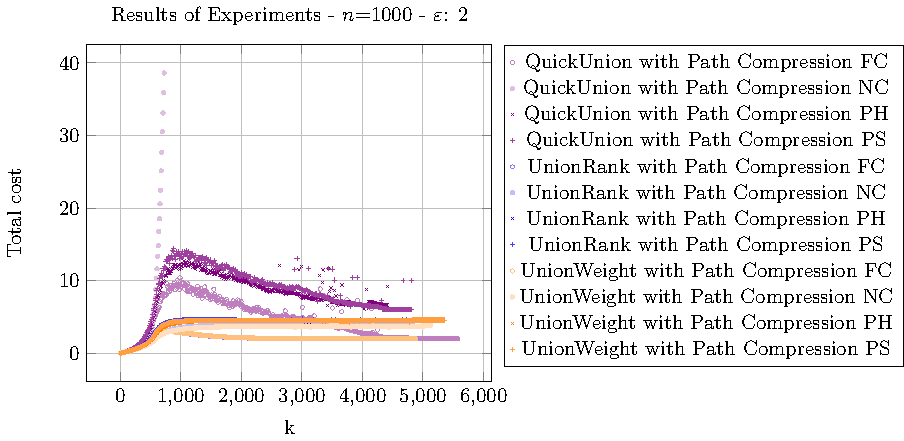
\includegraphics[width=\linewidth]{plots/plot_1000_Total_cost_epsilon_2.pdf}
            \caption{Total Cost for $n = 1000$ with $\varepsilon = 2$}
        \end{figure}
    \item[$\varepsilon = 4$] Same as above, but with $\varepsilon = 4$.
        \begin{figure}[h!]
            \centering
            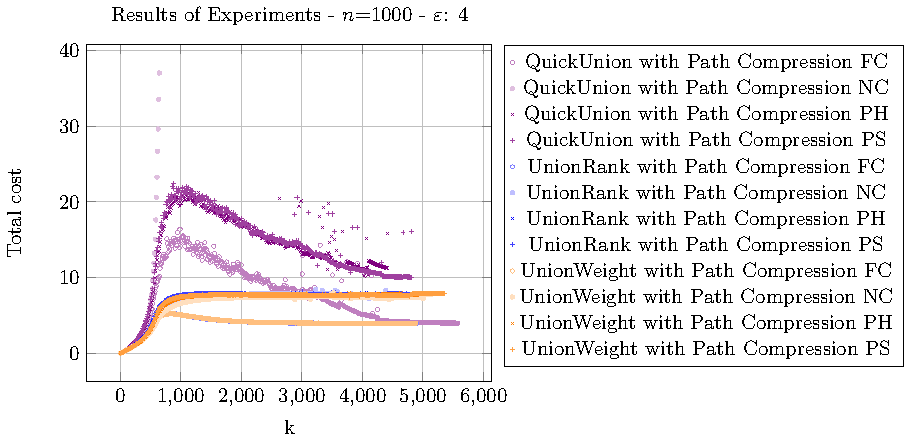
\includegraphics[width=\linewidth]{plots/plot_1000_Total_cost_epsilon_4.pdf}
            \caption{Total Cost for $n = 1000$ with $\varepsilon = 4$}
        \end{figure}
    \item[$\varepsilon = 8$] Same as above, but with $\varepsilon = 8$.
        \begin{figure}[h!]
            \centering
            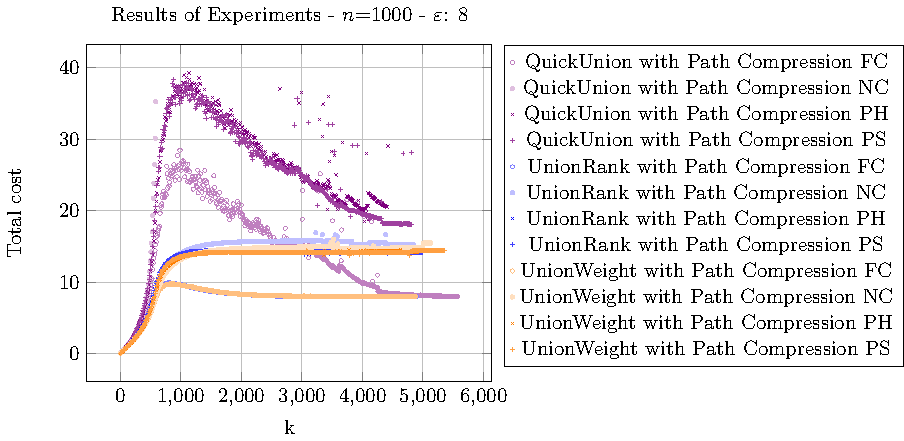
\includegraphics[width=\linewidth]{plots/plot_1000_Total_cost_epsilon_8.pdf}
            \caption{Total Cost for $n = 1000$ with $\varepsilon = 8$}
        \end{figure}
\end{description}

\section{Discussion}
This experiment
\section{Conclusion}


\newpage
\listoffigures
\lstlistoflistings
\listoftables


\end{document}
